\documentclass[10pt]{article}
\usepackage[english,russian]{babel}
\usepackage{textcomp}
\usepackage[left=2cm, right=2cm, top=1.5cm, bottom=1.5cm]{geometry}
\usepackage{tikz}
\usepackage{multicol}
\usepackage{hyperref}
\usepackage{amsmath}
\usepackage{listings}
\usepackage{colortbl}
\usepackage{graphicx}
\usepackage[shortlabels]{enumitem}
\usepackage{hyperref}
\pagenumbering{gobble}

\lstdefinestyle{CStyle}{
  language=C,
  basicstyle=\linespread{1.1}\ttfamily,
  basewidth=0.5em,
  texcl=true,
  keywordstyle=\color{blue}\bfseries,
  commentstyle=\color{gray},
  stringstyle=\ttfamily\color{orange!50!black},
  showstringspaces=false,
  backgroundcolor=\color{white},
  breaklines=true,
  breakatwhitespace=true,
  xleftmargin=5mm,
  keepspaces = true,
  extendedchars=\true,
  tabsize=4,
  upquote=true,
  emph={size_t, NULL},
  emphstyle={\color{blue}\bfseries},
}
\lstdefinestyle{boxStyle}{
  style=CStyle,
  framexleftmargin=5mm, 
  frame=shadowbox, 
  rulesepcolor=\color{gray}
}
\lstset{style=CStyle}

\renewcommand{\thesubsection}{\arabic{subsection}}
\makeatletter
\def\@seccntformat#1{\@ifundefined{#1@cntformat}%
   {\csname the#1\endcsname\quad}
   {\csname #1@cntformat\endcsname}}
\newcommand\section@cntformat{}
\newcommand\subsection@cntformat{Задача \thesubsection.\space}
\newcommand\subsubsection@cntformat{\thesubsubsection.\space}
\makeatother


\begin{document}

\title{Семинар \#7: Память и бинарные файлы. Домашнее задание.\vspace{-5ex}}\date{}\maketitle
\subsection{Просмотр памяти:}
Как выглядит память, инициализируемая при создании следующих переменных (в системе с порядком байт Little Endian):
\begin{itemize}
\item \texttt{int a = 0x11223344;}
\item \texttt{int b = 65535;}
\item \texttt{int c = -1;}
\item \texttt{int array[3] = \{10, 2000, 65535}\};
\item \texttt{char str[8] = '{}'Hello'{}'};
\item \texttt{float x = 1.0f};
\end{itemize}
Память представить в виде последовательности 2-значных шестнадцатеричных чисел. Например число \\
$123456_{10} = 1E240_{16}$ будет храниться в памяти как \texttt{40 E2 01 00}. Чтобы проверить, как будет выглядеть память, можно создать указатель типа \texttt{unsigned char*} на эту память и распечатать каждый байт в виде шестнадцатеричного числа.\\

Решение этой задачи -- это \texttt{.txt} файл, который будет содержать ответы на все подзадачи.


\subsection{Cat}
Что напечатает следующая программа и почему она это напечатает?
\begin{lstlisting} 
#include <stdio.h>
int main() 
{
    int a = 7627075;
    char* p = (char*)&a;
    printf("%s\n", p);
}
\end{lstlisting}

\subsection{Узнать порядок байт:}
Напишите функцию \texttt{int is\_little\_endian()} которая будет возвращать \texttt{1}, если эта функция запускается на системе с порядком байт Little Endian и \texttt{0}, если эта функция запускается на системе с порядком байт Big Endian.




\subsection{Запись массива чисел в файл}
Пусть у нас есть некоторый массив вещественных чисел:
\begin{lstlisting}
int n = 1000;
double* array = (double*)malloc(n * sizeof(double));

for (int i = 0; i < n; ++i)
    p[i] = sin(M_PI * i / n);
\end{lstlisting}

Напишите следующие функции, которые будут сохранять этот массив в файл:
\begin{itemize}
\item \texttt{void save\_numbers\_text(const char* filename, double* array, int n)} -- эта функция должна сохранять числа в файл в текстовом формате. Сначала эта функция должна записывать число \texttt{n}, а потом все числа с точностью в 15 знаков после запятой. Получившийся файл должен открываться с помощью текстового редактора.
\item \texttt{void save\_numbers\_binary(const char* filename, double* array, int n)} -- эта функция должна сохранять числа в бинарном формате. Сначала функция должна записывать количество чисел (в первые 4 байта файла), а потом она должна записывать сами числа, по 8 байт на одно число. 
\end{itemize}

\newpage
\subsection*{Рисование в файл изображения}
В дальнейших задачах вам понадобится программа для просмотра изображений в формате \texttt{ppm}. Если у вас нет программы, которая поддерживает этот  формат на компьютере, то советую использовать IrfanView: \href{https://www.irfanview.com/}{www.irfanview.com}.
В этой программе по умолчанию используется сглаживание при приближении. Его можно отключить, чтобы было видно каждый пиксель \texttt{View -> Display Options -> Use Resample for zooming} (убрать галочку).

\subsection{Флаг} 
В файле \texttt{flag.c} содержится пример работы создания изображения в формате \texttt{.ppm} в программе. Напишите программу, которая будет рисовать флаг Японии. Изображение должно иметь размер 600 на 400 пикселей. Компоненты белого цвета: \texttt{(255, 255, 255)}. Компоненты красного цвета: \texttt{(190, 0, 41)}.
\begin{center}
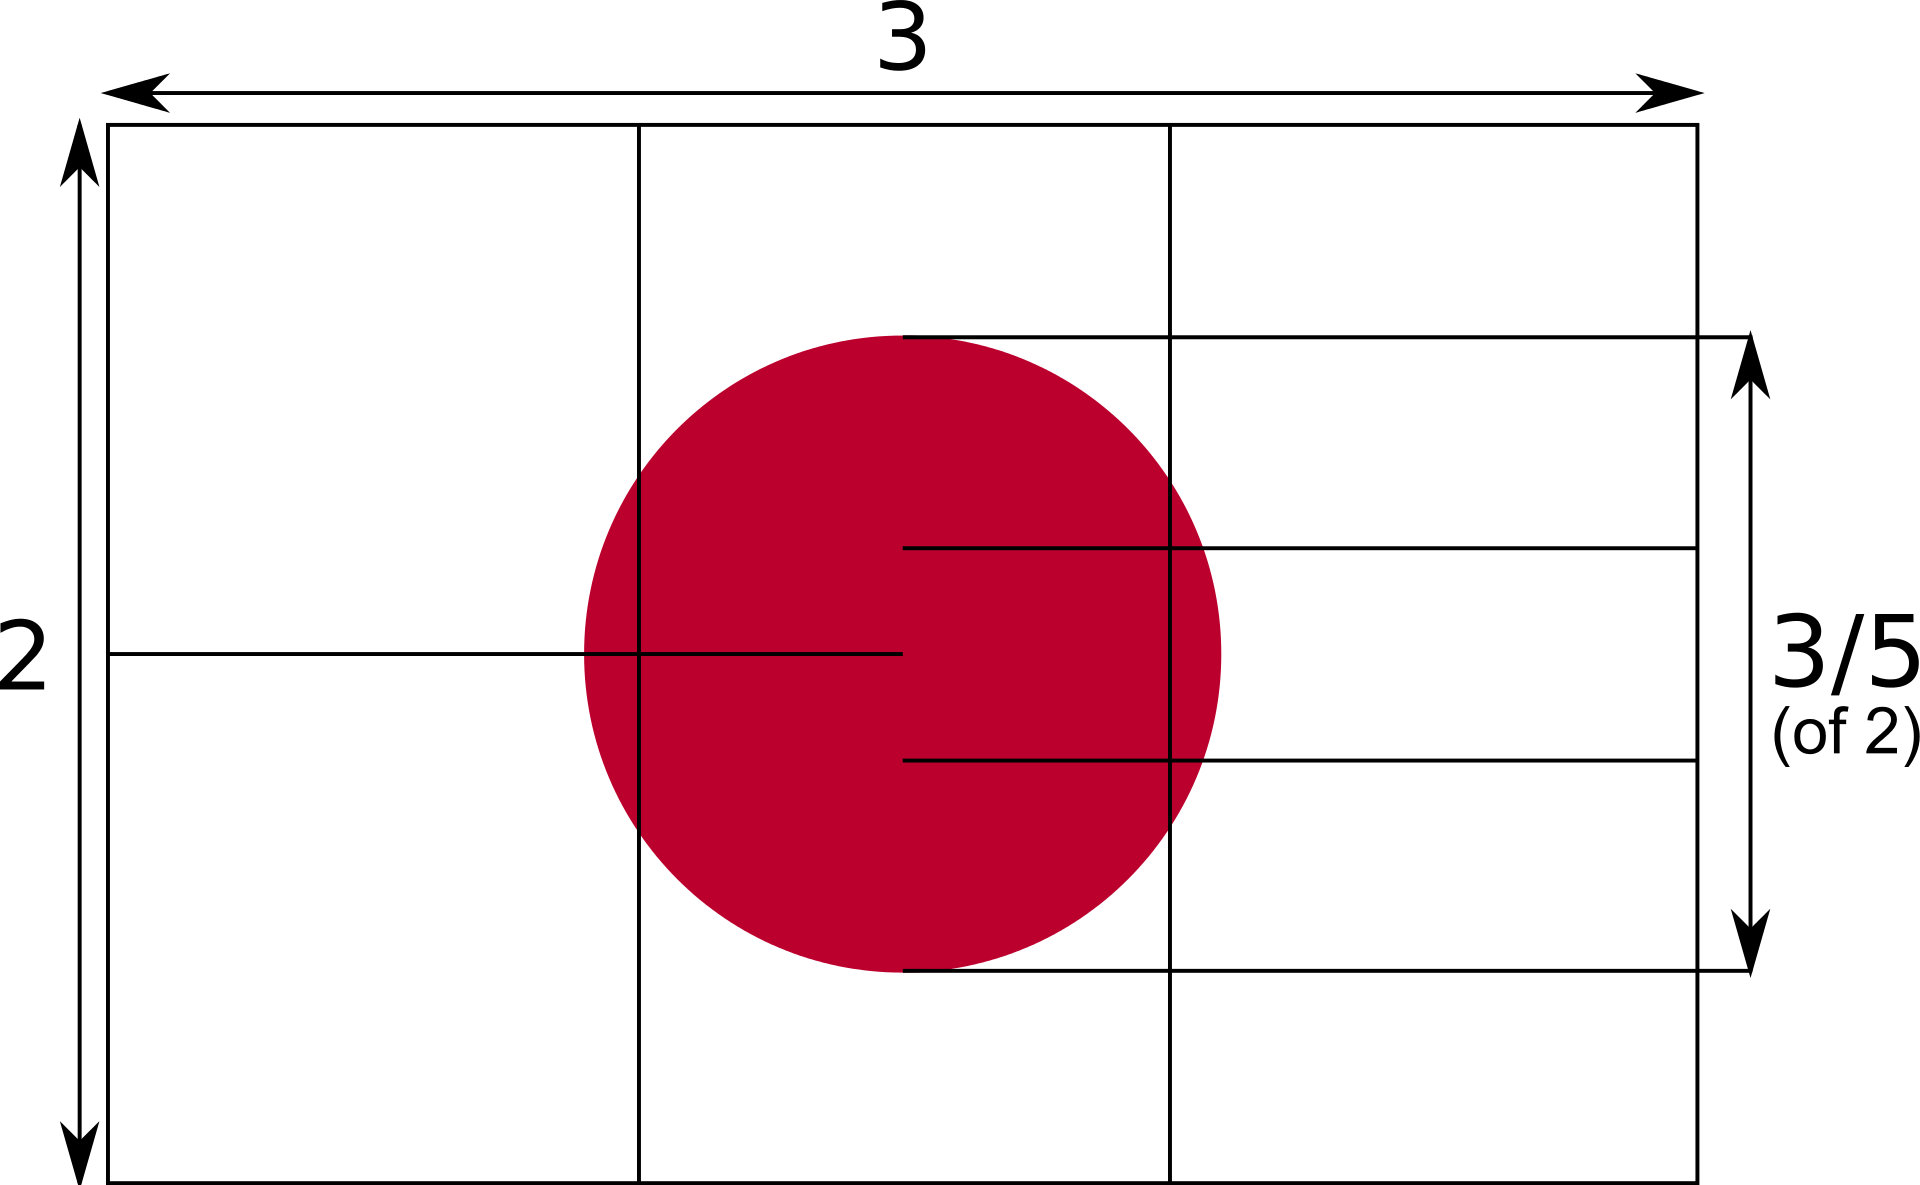
\includegraphics[scale=0.15]{../images/japanflag.png}
\end{center}

\subsection{Случайные круги} 
\begin{itemize}
\item Напишите функцию \\
\texttt{void draw\_circle(Color* data, int width, int height, int x0, int y0, int r, Color c)}\\
которая будет рисовать круг на холсте \texttt{data} с центром в точке \texttt{(x0, y0)}, радиусом \texttt{r} и цветом \texttt{c}.
\item Напишите программу, которая будет рисовать \texttt{n} кругов случайного цвета, расположения. Радиус тоже выбирается случайный в диапазоне от \texttt{a} до \texttt{b}. Параметры \texttt{n}, \texttt{a} и \texttt{b} передаются через аргументы командной строки. Программа должна создавать изображение \texttt{circles.ppm}.
\end{itemize}

\subsection{Функция двух переменных} 
Напишите программу, которая будет рисовать значения функции двух переменных $f(x, y)$ в области $[-1, 1]\times[-1, 1]$.\\
 Значения функции должны сохранятся в изображении размером 500 на 500 пикселей. К примеру, пиксель с координатами \texttt{(250, 250)} должен хранить значение функции в точке $(0, 0)$, а пиксель \texttt{(0, 400)} - значение в точке $(-1, 0.6)$. \\
Учтите, что значения пикселей изображения должны лежать в интервале от 0 до 255. Постройте изображения следующих функций: 
\begin{enumerate}
\item $f(x, y) = k\cdot|x \cdot y|$
\item $f(x, y) = k\cdot|sin(10\cdot(x^2 + y^2))|$
\item $f(x, y) = k\cdot|sin(5000\cdot(x^2 + y^2))|$
\item $f(x, y) = k\cdot|cos(10x)\cdot sin(10y)|$
\item $f(x, y) = k\frac{1}{2}\cdot\Big|sin\Big(\frac{3}{0.1 + |x|}\Big) + sin\Big(\frac{3}{0.1 + |y|}\Big)\Big|$
\end{enumerate}
Параметр $k = 255$ подбирается так, чтобы значения компонент цвета лежало в диапазоне от 0 до 255.


\subsection*{Обработка изображений}
В файле \texttt{brightness.c} содержится программа, которая увеличивает яркость изображения. Используйте её как пример для решения следующих задач. Компиляция и запуск этой программы осуществляется следующим образом:
\begin{verbatim}
gcc -std=c99 -o brighter brightness.c
./brighter images/emir.ppm 50
\end{verbatim}

\subsection{Черно-белое изображение} 
Написать программу, которая принимает на вход файл изображения, считывает его и превращает в чёрно-белое изображение и записывает в файл \texttt{result.ppm}. Название изображения должно передаваться через аргументы командной строки.

\subsection{Перестановка цветов:} Написать программу, которая переставляет местами красную и синюю компоненты цвета. Применить её на файле \texttt{emir.ppm}.



\subsection{Сепия} 
Написать программу, которая будет применять к изображению эффект сепии.
\begin{multicols}{3}
Формулы для эффекта сепии:
\begin{align*}
r_{new} = 0.393 \cdot r + 0.769 \cdot g + 0.189 \cdot b\\
g_{new} = 0.349 \cdot r + 0.686 \cdot g + 0.168 \cdot b\\
b_{new} = 0.272 \cdot r + 0.534 \cdot g + 0.131 \cdot b\\
\end{align*}
Если какое-то из этих значение станет большим, чем $255$, то его нужно приравнять к $255$.
\vfill			
\begin{center}
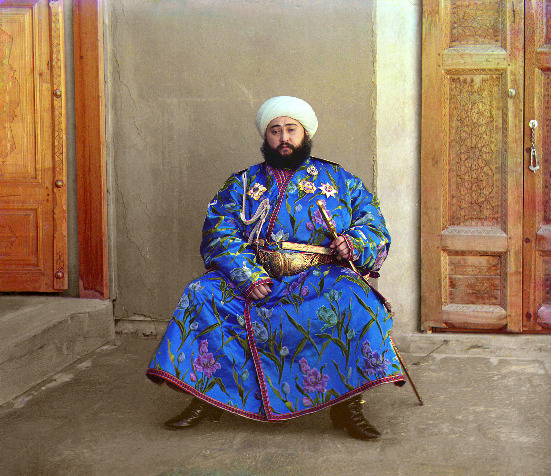
\includegraphics[scale=0.26]{../images/imageproc.jpg}
\end{center}
\vfill			
\begin{center}
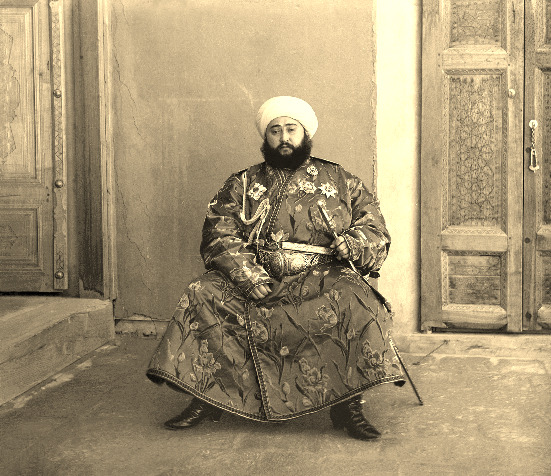
\includegraphics[scale=0.26]{../images/imageproc_sepia.jpg}
\end{center}
\end{multicols}


\subsection{Свёртка изображения.}
Операция свёртки изображения задаётся следующей формулой:
\begin{align*}
data_{new}[i, j] = \sum_{p=-1}^{1} \sum_{q=-1}^{1} K[p+1, q+1] \cdot data[i+p, j+q]\\
\end{align*}
, где $K$ - некоторая матрица 3 на 3. Для размытия эта матрица равна:
$$
K = 
\frac{1}{9}
\begin{pmatrix}
1 & 1 & 1 \\
1 & 1 & 1 \\
1 & 1 & 1
\end{pmatrix}
$$\\

Подробней о свёртке можно посмотреть тут:
 \href{https://www.youtube.com/watch?v=C_zFhWdM4ic&t=74s}{\texttt{www.youtube.com/watch?v=C\_zFhWdM4ic}}\\
Если провести эту операцию 1 раз, то размытие будет небольшое. Чтобы размыть изображение сильнее нужно повторить эту операцию несколько раз.
Напишите программу, которая будет размывать изображение \texttt{n} раз (\texttt{n} передаётся через аргументы командной строки).


\iffalse
\item \textbf{Нахождение границ:} Для нахождения вертикальных или горизонтальных границ на изображении, сначала нужно превратить это изображение в черно-белое, а затем применить свёртку со следующей матрицей:
\begin{multicols}{2}
$$
K_1 = 
\frac{1}{k}
\begin{pmatrix}
-1 & 0 & 1 \\
-2 & 0 & 2 \\
-1 & 0 & 1
\end{pmatrix}
$$\\
\vfill
$$
K_2 = 
\frac{1}{k}
\begin{pmatrix}
1 & 2 & 1 \\
0 & 0 & 0 \\
-1 & -2 & -1
\end{pmatrix}
$$\\
\end{multicols}
Параметр $k$ настраивается. Обычно $k \approx 50$.\\
Изображение, содержащее все границы находится применением оператора $K = \sqrt{K_1^2 + K_2^2}$.
\fi


\newpage
\subsection*{Рисование линий. Алгоритм Брезенхема:}
Алгоритм построения прямой линии между двумя точками на двумерном холсте называется алгоритмом Брезенхема.
В файле \texttt{4lines.c} есть реализация этого алгоритма на языке \texttt{C}.
\begin{center}
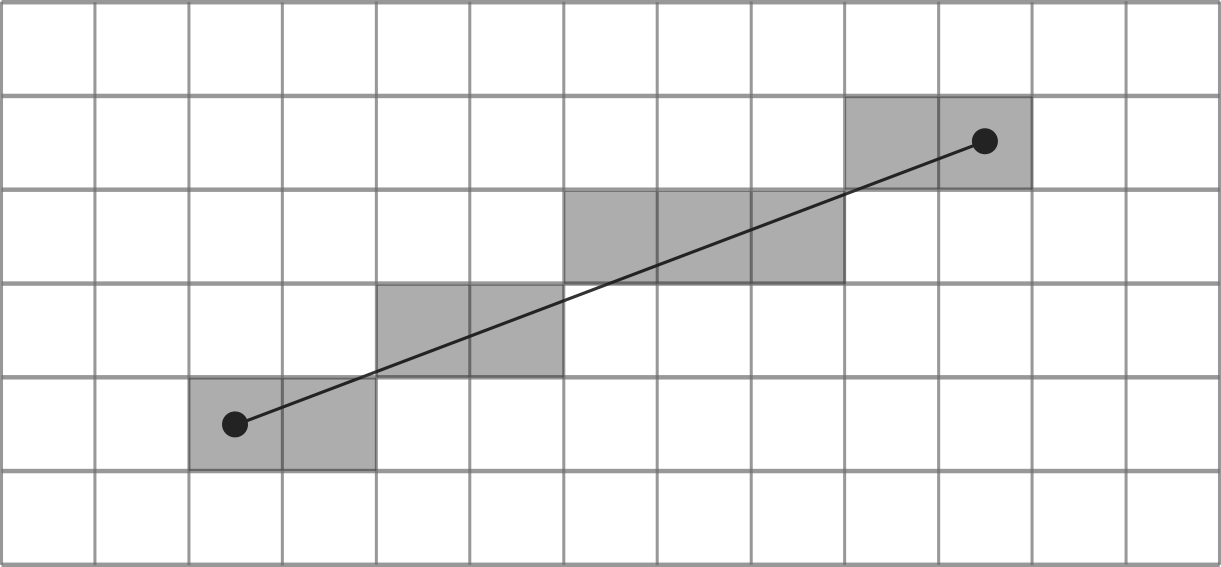
\includegraphics[scale=1]{../images/bresenham.png}
\end{center}

\subsection{Случайные линии}
Создать программу, которая будет рисовать \texttt{n} случайных отрезков случайного цвета. \texttt{n} должен передаваться через аргументы командной строки. Программа должна создавать файл \texttt{randlines.ppm}.

\subsection{Фрактальное дерево:}
Напишите рекурсивную функцию, которая будет рисовать фрактальное дерево:
\begin{center}
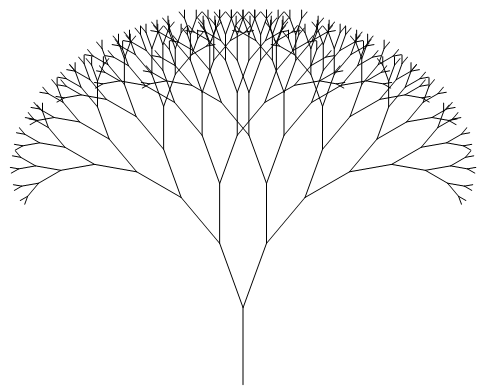
\includegraphics[scale=0.4]{../images/treefractal.png}
\end{center}

\newpage
\subsection*{Работа с изображениями формата \texttt{.jpg} с помощью библиотеки stb}

\subsection{Консольный графический редактор:} Объедините все решения предыдущих задач в одну программу \texttt{mge}. Выбор эффекта должен задаваться с помощью аргументов командной строки. Например так:
\begin{verbatim}
mge --sepia image.ppm result.ppm
\end{verbatim}
Программа должна применять эффект сепии на изображение \texttt{image.ppm} и сохранять результат в \texttt{result.ppm}.

А при таком вызове программа должна применять эффект размытия 10 раз:
\begin{verbatim}
mge --blur 10 image.ppm result.ppm
\end{verbatim}
Добавьте ещё опции: \texttt{----brighter}, \texttt{----bw}, \texttt{----changecolors}, \texttt{----mirror}.

\end{document}
